\chapter{Numerical Results}

\section{Alterable Schedule}

\subsection{State (3, 2)}

Assume that the mean service time $\mu$ is $1$. In addition, assume that the per unit time costs of the customers' waiting time and server's idle time ($c_{W}$ and $c_{I}$ respectively) are both $1$. Under these assumptions, the cost of state $(3, 2)$ for various values of $a$ is given by the following expression, which is continuous for $a \geq 0$.

\begin{equation*}
	C_{3} (a, 2) =
	\begin{cases}
 		9.88121 & \text{where $a = 0$} \\
 		\frac{\mathrm{e}^{-a} \left( \mathrm{e}^{a} a (2.29362 - 0.5 a) - (0.5 a + 3.29362) a - 1.15888 \mathrm{e}^{a} + (a + 5.52005) \mathrm{e}^{2 a} - 4.36117 \right)}{\mathrm{e}^{a} - 1} & \text{where $a > 0$}
	\end{cases}
\end{equation*}

This equation is plotted for $a \in [0, 10]$ to visualise the relationship between the cost and $a$. The resulting figure is Figure \ref{Graph_3_2}.

\begin{figure}[h]
	\centering
	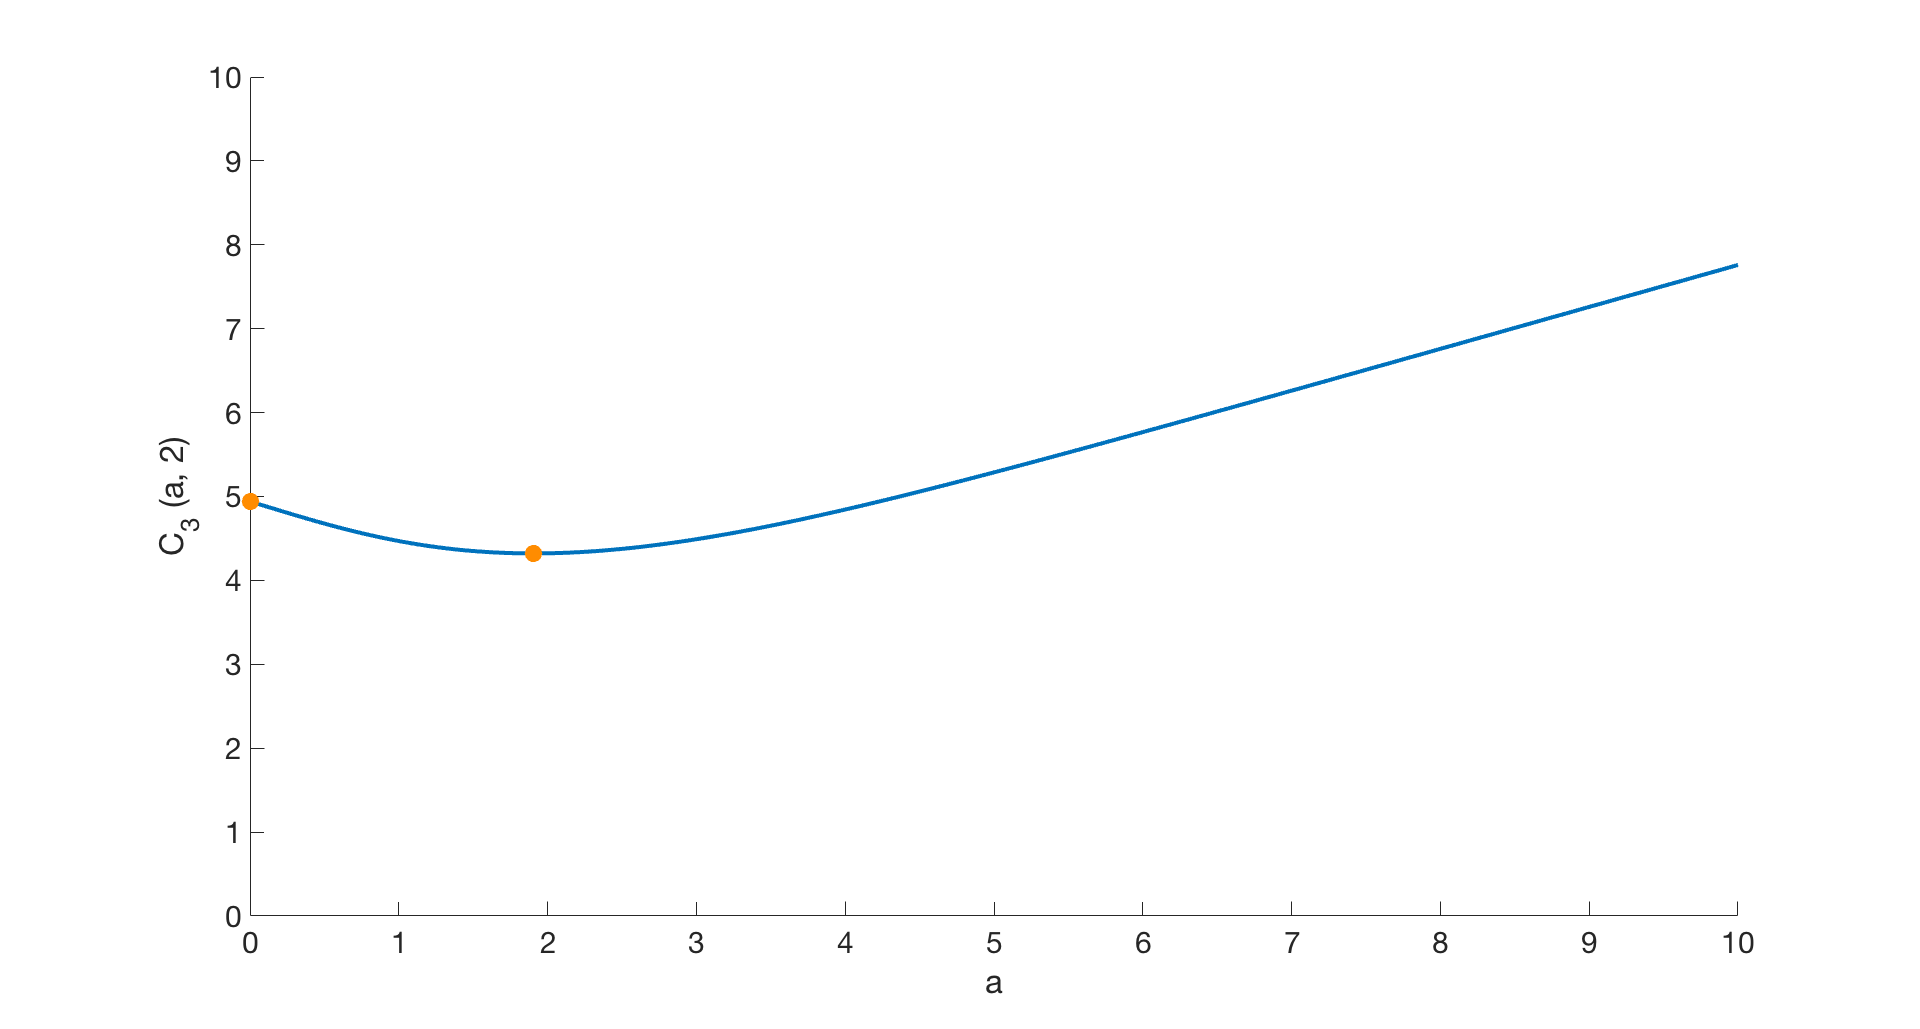
\includegraphics[width = 0.85\textwidth]{Graph_3_2.png}
	\caption{Cost of state with n = 3, k = 2 for various values of a}
	\label{Graph_3_2}
\end{figure}

The only value of $a$ where $\frac{\partial}{\partial a} C_{3} (a, 2) = 0$ is $a = 1.90481$. Thus, the set of possible policies is $\mathcal{A} = \{ 0, 1.90481 \}$ whereby there are two possible policies labelled as orange dots on Figure \ref{Graph_3_2}. Moreover, note that as $a$ increases beyond 2, the cost increases approximately linearly as the expected waiting time of the next customer and the expected idle time of the server both increase linearly.

The optimal policy $a^{*}$ that minimises $C_{3} (a, 2)$ is $1.90481$ where the cost is $8.64338$. If on arrival of a customer, there are $2$ customers in the queue and $3$ customers remaining to be scheduled, then the next customer should be scheduled to arrive in $1.90481$ time units. This is slightly below the expected service time of the two customers in the queue to account for the idle cost of the server.

\subsection{6 Customers}